\documentclass[12pt]{article}

\usepackage[margin=1in, top=1in, bottom=1in]{geometry}

\usepackage{amsmath,amssymb,amsthm,epsfig,rotfloat,psfrag,natbib,url,graphicx,lineno}
\usepackage[color=white]{todonotes}
%\usepackage{authblk}

\newcommand{\cmt}[1]{\todo[inline]{\color{blue} {\sc Comment:} \newline #1}}

% \usepackage{fourier}

%%%%
% Some shortcut notation
%%%%
  \newcommand{\by}{\mathbf{y}}
  \newcommand{\bt}{\boldsymbol{\theta}}
  \newcommand{\bvt}{\boldsymbol{\vartheta}}
  \newcommand{\bb}{\boldsymbol{\beta}}
  \newcommand{\bn}{\boldsymbol{\eta}}
  \newcommand{\bT}{\boldsymbol{\Theta}}
  \newcommand{\bp}{\boldsymbol{\psi}}
  \newcommand{\bP}{\boldsymbol{\Psi}}
  \newcommand{\bg}{\boldsymbol{\gamma}}
  \newcommand{\bG}{\boldsymbol{\Gamma}}
  \newcommand{\be}{\boldsymbol{\epsilon}}
  \newcommand{\bm}{\boldsymbol{\mu}}
  \newcommand{\bSig}{\boldsymbol{\Sigma}}
  \newcommand{\bO}{\boldsymbol{\Omega}}
  \newcommand{\ba}{\boldsymbol{\alpha}}
  \newcommand{\bxi}{\boldsymbol{\xi}}
  \newcommand{\bS}{\mathbf{S}}
  \newcommand{\bL}{\mathbf{L}}
  \newcommand{\bK}{\mathbf{K}}
  \newcommand{\bX}{\mathbf{X}}
  \newcommand{\bQ}{\mathbf{Q}}
  \newcommand{\bV}{\mathbf{V}}
  \newcommand{\bZ}{\mathbf{Z}}
  \newcommand{\fD}{\mathcal{D}}
  \newcommand{\fY}{\mathcal{Y}}
  \newcommand{\bu}{\mathbf{u}}
  \newcommand{\tN}{\text{N}}
  \newcommand{\bY}{\mathbf{Y}}
  \newcommand{\bI}{\mathbf{I}}
  \newcommand{\bz}{\mathbf{0}}
  
  
\bibliographystyle{apalike2}


\begin{document}
%\vspace*{0.15\textheight}

\vspace*{\fill}

\begin{center}
\setlength{\parindent}{0pt}
\renewcommand{\baselinestretch}{1.8}\normalsize

{\Large Greater Than the Sum of its Parts: Computationally Flexible Inference for Bayesian Hierarchical Models}

\renewcommand{\baselinestretch}{1.15}\normalsize 
\bigskip\bigskip

Devin S. Johnson\footnote{Corresponding author: {\tt devin.johnson@noaa.gov}}\\ 
Alaska Fisheries Science Center,\\
National Marine Fisheries Service, NOAA \medskip

and\medskip

Brian M. Brost\\
Alaska Fisheries Science Center,\\
National Marine Fisheries Service, NOAA \medskip

and\medskip

Mevin B. Hooten \\
U.S. Geological Survey\\
Colorado Cooperative Fish and Wildlife Research Unit\\
Department of Fish, Wildlife, and Conservation Biology\\
Department of Statistics\\
Colorado State University

\bigskip\bigskip

\today

\end{center}

\vspace*{\fill}

\clearpage

%\renewcommand{\baselinestretch}{1.5}\normalsize

%% ABSTRACT %%%%%%%%%%%%%%%%%%%%%%%%%%%%%%%%%%%%%%%%%%%%%%%%%%%%%

\vspace*{\fill}
\begin{center}
\begin{minipage}{0.65\paperwidth}
\renewcommand{\baselinestretch}{1}\normalsize

\centerline{\bf Abstract} 
We propose a multistage method for making inference at all levels of an BHM using natural data partitions to increase efficiency by allowing computations to take place in parallel form using whatever software is most appropriate for each data partition. The full hierarchical model is then approximated by the product of independent normal distributions for the data component of the model. In the second stage, the Bayesian MAP estimator is found my maximizing the approximated posterior density with respect to the parameters. If the parameters of the model can be represented as normal distributed random effects then the second stage optimization is equivalent to fitting a multivariate normal linear mixed model. This method can be extended to account for common fixed parameters shared between data partitions, as well as, parameters that are distinct in purpose between partitions. In the case of distinct parameter estimation we consider a third stage which re-estimates the distinct parameters for each data partition based on the results of the second stage. This allows more information from the entire data set to properly inform the posterior distributions of the distinct parameters. The method is demonstrated with two ecological data sets and models: a random effects GLM and an Integrated Population Model (IPM). Standard GLM software available in the {\tt R} was used in the first stage of the GLM analysis, while multiple software platforms were used for the IPM analysis. In both examples the {\tt R} package {\tt TMB} was used to fit the second stage linear mixed model. The multistage results were compared to estimates from models fit in single stages to the entire data set. Both examples demonstrate that multistage point and posterior standard deviation estimates are very close those obtained from fitting the models with all data simultaneously and can therefore be considered for fitting hierarchical Bayesian models when it is computationally prohibitive to do so in one step.     

\bigskip

{\bf Key words}: Approximation; Bayesian MAP estimation; Bayesian Hierarchical Model; Integrated Population Model; Linear mixed model; Meta-analysis; Multistage estimation
\end{minipage}
\end{center}

\vspace*{\fill}

\clearpage

\renewcommand{\baselinestretch}{1.5}\normalsize
\raggedright
\setlength{\parindent}{2em}
\raggedbottom
\linenumbers

\section{Introduction}

\cmt{Here's a comment if you want to say something}

Bayesian hierarchical models (BHMs) have become ubiquitous in most fields of scientific enquiry because of their ability to flexibly model complex natural systems yet remain relatively easy to build and modify for the questions at hand \citep{hobbs2015bayesian}. The influential paper of \cite{berliner1996hierarchical} set up a general description of a BHM based on three submodels: (1) {\it data}, (2) {\it process}, and (3) {\it parameter} models. The data model accounts for measurement error or other differences between observable data and the true natural process for which the researcher would like to make inference. The process model describes the state of nature using a random process to account for its unknown intricacies. Finally, the parameter model describes our uncertainty about the parameters governing this random process.  The full model is built by conditioning each submodel on the one above it. Traditionally, inference for BHMs has been conducted using some form of Markov Chain Monte Carlo (MCMC) because the model structure is ideally suited to it \citep{gelfand1990sampling,gelfand2015hierarchical}. If not for development of MCMC methods, widespread use of BHMs may never have come to pass \citep{green2015bayesian}. With a large amount of data or complex submodels, however, MCMC can be computationally challenging or infeasible to implement \citep{hooten2018prior, wikle2003hierarchical}. Herein, we propose a multistage method for making inference at all levels of an BHM using various various software formats in each stage. By breaking the estimation procedure into multiple stages based on partition of the full data it becomes very computationally efficient. By allowing whichever software platform is most efficient in the initial stage it can be made more efficient yet, not only in computer time, but also real human time that can be saved by using software designed to facilitate each specific initial stage analysis. 

To combat computational challenges in using MCMC to fit BHMs in ``big data'' situations there have been several avenues of approach  developing in the literature. One of these, is development of so called ``2-stage'' methods. These methods seek to break the computations into pieces based on partitions of the data \citep{goudie2019joining, hooten2016hierarchical,hooten2018prior,lunn2013fully,mesquita2020embarrassingly}. The first stage involves fitting separate data models to the partitions using MCMC, then in the second stage the separate MCMC samples are combined to produce an MCMC sample as if the partitions had been simultaneously analyzed with the full BHM. Before the wide-spread use of MCMC \cite{kass1989approximate} considered a 2-stage estimation method for a specific class of HMBs known as {\it conditionally independent hierarchical models} (CIHMs). In these models data partitions are conditionally independent given parameter values. In another example of 2-stage inference for an BHM without MCMC, \citet{burnham2002evaluation} used meta-analysis methods to fit random effects models for capture-recapture survival data. Meta-analysis methods are designed as a 2-stage analysis where results of many separate analyses are combined using a linear mixed model to describe population average effects and account for estimation uncertainty in the first stage \citep{gasparrini2012multivariate,higgins2009re}. 

A second alternative approach to default MCMC for computationally challenging BHMs is to not use posterior sampling all, instead use  optimization methods for exploring the posterior parameter space \citep{green2015bayesian}. Optimization of the posterior density aims to find the  {\it maximum a posteriori} (MAP) estimate rather than the posterior mean. The main benefit is that optimizing the posterior with respect to the parameters often requires fewer evaluations of the posterior density. The come at a cost , however, because asymptotic results are usually required to describe parameter uncertainty \citep{van2000asymptotic}. The development of automatic differentiation software has aided the development of efficient optimization inference for BHMs \citep{kristensen2016tmb, skaug2006automatic}.

In an effort to provide a computationally efficient and flexible method for fitting HMBs, specifically, CIHMs, we consider combining benefits of meta-analysis, 2-stage MCMC, and posterior optimization into a multistage method that can be used to quickly fit BHMs in big data situations or when the data level models are complex in their own right. Although meta-analysis and 2-stage MCMC are both accomplished in multiple stages, 2-stage MCMC is initially designed to analyze an BHM, whereas meta-analysis seeks to summarize results from various analyses by forming them into an BHM, namely, a multivariate normal linear mixed model \citep{gasparrini2012multivariate}. We can use the meta-analysis approach to approximate the second stage combination of initial stage inference in a 2-stage MCMC. This allows us to use multiple different methods to approximate the posterior inference in the initial stage, including optimization methods, deterministic sampling, or MCMC if it is convenient. 

The paper proceeds by providing notation and a working definition of the CIHM as we will use it. In the following section we show how the full posterior can be approximated using multivariate normal approximations to first stage posterior densities. Then we demonstrate the how the initial stage results can be combined using the linear mixed model approach of standard meta-analysis when the first stage parameters are random effects. We extend the method for estimating all types of parameters in the full CIHM. A third stage is introduced to retroactively revisit the first stage analysis and improve some estimates after the second stage results are obtained. The method is then demonstrated for two different types of environmental data, a simple generalized linear mixed model (GLMM) and an integrated data model for Bayesian melding. 


\section{Methods}

The description of BHMs by \cite{berliner1996hierarchical} is very general and we only consider a specific, but still very broad, class of hierarchical models here, {\it Conditionally independent hierarchical models} (CIHM; \citealt{kass1989approximate,gelfand2015hierarchical}). However, in the Discussion section we note that some of these assumptions about model form and distribution can be relaxed. The general form of a CIHM model is
\begin{equation}\label{eq:full.model}
\begin{aligned}
\text{Data-level model: } & \bY = \{\by_1,\dots,\by_n\} \sim \prod_{i=1}^n[\by_i|\bt_i, \bg_i, \bn] \\
\text{Unit-level effects: } & \bT = \{\bt_1,\dots,\bt_n\} \sim \prod_{i=1}^n[\bt_i|\bp]\\
 & \bG = \{\bg_1,\dots,\bg_n\} \sim \prod_{i=1}^n[\bg_i] \\
\text{Population effects: } & \bP = \{\bp,\bn\} \sim [\bp,\bn],
\end{aligned}
\end{equation}
where ``$[A|B]$'' is used to represent the conditional probability density or distribution function of $A$ given $B$ \citep{gelfand1990sampling}, $\by_i$ is the observed data set (or data partition) for the $i$th unit, $\bt_i$ are unit-level parameters, governed by $\bp$, population-level parameters, $\bg_i$ are distinct parameters for for modeling the $i$th data set, and $\bn$ are global (fixed) population level parameters. Typically, $\bp$ and $\bn$ are the most scientifically interesting, however, there can be interest in each of the $\bt_i$ and $\bg_i$ depending on the situation. Note, that the different data sets do not need to contain the same type of data, that is the units are not necessarily exchangeable individuals. Combing data via a BHM is often termed ``Bayesian melding''  \citep{goudie2019joining, liu2014bayesian}. See Section 4 for an example. While this class of BHMs is large, in the discussion in Section 5, we will how this method can be expanded beyond CIHMs.


\subsection{Two-stage approximate Bayesian inference}

We begin our investigation of two-stage model fitting with individual based hierarchical models. We will initially assume that the data-level models can be written as $[\by_i|\bt_i, \bg_i, \bn]=[\by_i|\bt_i]$, that is, either there are no fixed parameters, or they can be absorbed into $\bp$ via, say, hierarchical centering \citep{Gelfand:1996zq}. We will return to general CIHM model in the following section. 

If we were to fit this model in the traditional way we would use summaries from the full posterior distribution 
\[
[\bp, \bT|\bY] \propto \left(\prod_i[\by_i|\bt_i][\bt_i|\bp]\right) [\bp].
\]
Using this type of hierarchical model in the presence of individual heterogeneity has many beneficial qualities for accurately assessing uncertainty when population-level inference is the main scientific interest \citep{Cressie:2009rr}. However, with modern data collection technology, the individual $\by_i$ data sets can become quite large and if evaluating $[\by_i|\bt_i]$ is sufficiently complex, making inference to the full posterior distribution can become computationally challenging (e.g., \citealt{hooten2016hierarchical}).

To begin, suppose we are only in possession of a single $\by_i$, then we might estimate $\bt_i$ using the posterior distribution
\[
[\bt_i|\by_i] \propto [\by_i|\bt_i]\ [\bt_i],
\]
where $[\bt_i]$ is a prior distribution that would be used in the absence of additional individuals. We can accurately interpret this posterior as all of our knowledge about $\bt_i$ given $\by_i$ (and choice of $[\bt_i]$, but we address this momentarily). Using the individual posterior distributions, we can rewrite the full hierarchical model posterior as 
\begin{equation}
\label{eq:post}
\begin{aligned}[]
[\bp,\bT|\bY] &\propto [\bY|\bT]\ [\bT|\bp]\ [\bp]\\
& \propto \left(\prod_{i=1}^n\frac{[\bt_i|\by_i]}{[\bt_i]}\ [\bt_i|\bp]\right)\ [\bp].
\end{aligned}
\end{equation}
As the reader can see, once the data has been summarized into the posteriors the likelihood is not needed, per se, for full hierarchical modeling. 

When evaluating the posterior distribution in equation (\ref{eq:post}), the individual posteriors, $[\bt_i|\by_i]$ are typically not available in closed form. Many times one may fit an individual model with Markov Chain Monte Carlo (MCMC), therefore, $[\bt_i|\by_i]$ is represented by a stochastic sample. The method proposed by \citet{lunn2013fully} is useful for this situation. Here we explore an alternative approach when optimization can be used to find the individual posteriors.

The initial stage (``stage I'') of the method we propose begins by first optimizing $[\bt_i|\by_i]/[\bt_i]$ = $[\by_i|\bt_i]$ with respect to $\bt_i$ for each data set or partition. Of course, this just results in the maximum likelihood estimate (MLE) $\hat{\bt}_i$ for the data $\by_i$. Then if the data is informative enough, we can approximate 
\[
\frac{[\bt_i|\by_i]}{[\bt_i]} \approx \text{N}(\bt_i|\hat{\bt}_i, \hat{\bS}_i)
\]
where $\hat{\bS}_i$ is the negative inverse Hessian of the log-likelihood. This is just the standard large-sample asymptotic results for an MLE. Without any further assumptions the desired posterior is thus approximated by
\begin{equation}
\label{eq:normpost}
[\bp,\bT|\bY] \approx  \prod_{i=1}^n\left(\text{N}(\hat{\bt}_i|\bt_i, \hat{\bS}_i)\ [\bt_i|\bp]\right)\ [\bp].
\end{equation}
Note that we have put $\bt_i$ in the mean position of the normal specification. Due to the symmetry of the normal density function it is equivalent, but this way $\hat{\bt}_i$, can be interpreted as an observation while $\bt_i$ retains its random effect interpretation. In essence, the information in the original likelihood, $[\by_i|\bt_i]$ about $\bt_i$ was compressed into the approximate likelihood $\text{N}(\hat{\bt}_i|\bt_i, \hat{\bS}_i)$. The benefit of stage I is that this compression can be accomplished separately and in parallel for each unit. In ``stage II'', we can make full inference for all model parameters by maximizing the approximate full posterior (\ref{eq:normpost}) to obtain the posterior mode $(\tilde{\bp},\tilde{\bT})$, or {\it maximum a posteriori} (MAP) estimate and the negative inverse Hessian of the log posterior density estimates posterior covariance matrix. Herein we will use hats to represnet stage I estimates and tildes to represent stage II estimates.

While we have painted a rather straightforward picture of the method so far, in practice, there exists the possibility that $\bt_i$ is only weakly identified in $[\by_i|\bt_i]$. Using the complete data, $\bY$, within the hierarchical model provides the information necessary to identify $\bt_i$. So, maximizing the posterior $[\bt_i|\by_i] = [\by_i|\bt_i][\bt_i]$ might be necessary, where $[\bt_i]$ is chosen to make all parameters identifiable. Because we are free to choose the temporary prior to aid stage I model fitting, we suggest using a normal prior
\[
[\bt_i] = \text{N}(\bt_i|\bt_0, \bS_0)
\]
A reparameteriztion of $\bt_i$ might be necessary such that a normal density is appropriate as a prior, but this will only help the normal approximation in stage I anyway. Now with the use of the temporary prior the approximation becomes \citep{goudie2019joining},
\begin{equation}
\label{eq:pseudo.prior}
\frac{[\bt_i|\by_i]}{[\bt_i]} \approx \frac{\text{N}(\bt_i|\Check{\bt}_i, \Check{\bS}_i)}{\text{N}(\bt_i|\bt_0, \bS_0)} \propto \text{N}(\bt_i|\hat{\bt}_i, \hat{\bS}_i),
\end{equation}
where,
\begin{equation}
\label{eq:pprior.remove}
\hat{\bS}_i = \left(\Check{\bS}_i^{-1} - \bS_0^{-1}\right)^{-1} 
\ \ \text{and}\ \ 
\hat{\bt}_i = \hat{\bS}_i \left(  \Check{\bS}_i^{-1}\Check{\bt}_i -  \bS_0^{-1}\bt_0\right),
\end{equation}
where $\Check{\bt}_i$ and $\Check{\bS}_i$ are the MAP and large sample covariance matrix of $\log [\by_i|\bt_i][\bt_i]$. Thus, we can still use the same form (\ref{eq:normpost}) as before, one just needs to remove the effect of the temporary prior for stage II estimation. 


\subsection{Normal random effects models}

In this section we focus on the usual case of normally distributed random effects. While there is no requirement that $\bT$ be normally distributed in (\ref{eq:normpost}), this probably accounts for the vast majority of applications. For many applications $\bt_i$ can be parameterized such that a normal distribution is appropriate. So, for the remainder of the paper, we will assume that, 
\[
[\bt_i|\bb, \bSig] = \text{N}(\bt_i|\bX_i\bb, \bSig).
\]
When this is the case, stage II becomes equivalent to fitting a multivariate normal random effects regression model. 

First we reparameterize the model using $\bt_i = \bX_i\bb + \bu_i$ where $[\bu_i|\bSig] = \tN(\mathbf{0},\bSig)$. Now, the posterior of interest is approximated with
\begin{equation}
\label{eq:normeff}
[\bb,\bSig,\bu|\bY] \approx  \prod_{i=1}^n\left(\tN(\hat{\bt}_i|\bX_i\bb+\bu_i, \hat{\bS}_i)\cdot \tN(\bu_i|\mathbf{0},\bSig)\right)\ [\bb, \bSig].
\end{equation}
This, of coarse, is equal to the multivariate linear mixed model
\[
\hat{\bt}_i = \bX_i\bb + \bu_i + \boldsymbol{\epsilon}_i
\]
with random effect $\bu_i \sim \text{N}(\mathbf{0},\bSig)$ and error $\boldsymbol{\epsilon}_i \sim \text{N}(\mathbf{0},\hat{\bS}_i)$. We can write this in full matrix form as:
\begin{equation}\label{eq:full.mat.form}
\hat{\bt} = \bX\bb + \bu + \boldsymbol{\epsilon}
\end{equation}
where all the model terms are concatenated, $\hat{\bt} = (\hat{\bt}_1',\dots,\hat{\bt}_n')'$, $\bX = (\bX_1',\dots,\bX_n')'$, $\bu \sim \tN(\bz, \bI_n\otimes\bSig)$, and $\boldsymbol{\epsilon} \sim \tN(\mathbf{0}, diag(\hat{\bS}_1,\dots,\hat{\bS}_n))$. We use the notation `$diag(\dots)$' to represent a block-diagonal matrix build from the arguments. 

This is how random effects meta-analysis is most often considered \citep{higgins2009re}. Traditionally, a restricted maximum likelihood (REML) estimate of the variance terms combined with generalized least-squares estimate of the fixed effects, $\bb$, is used to estimate parameters and perform predictions, $\bt^*_i = \bX_i\bb + \hat{\bu}_i$. Both \citet{burnham2002evaluation} and \cite{zeppelin2019migratory} demonstrate the REML approach for fitting a random effects BHM. However, the usual REML approach does not full account uncertainty of the variance estimates in these predictions, other estimation methods, such as MCMC are necessary. We use the {\tt R} package {\tt TMB} to fit (\ref{eq:normeff}). A Laplace approximation is used to integrate over $\bu$, then a generalized delta-method is employed to estimate $\bu$ accounting for uncertainty in the other parameters \citep{kristensen2016tmb,skaug2006automatic}. 






\subsection{Modeling fixed effects and distinct parameters}

Now that we have considered the case of a random effects only data model, we return to the case where there are distinct individual effects ($\bg_i$) and global fixed parameters ($\bn$) in the data model that cannot be easily reparameterized to higher levels in the hierarchy. At first glance, these parameters might seem different but they can both be considered as population-level fixed effects. Let $\bvt_i = (\bt_i', \bn', \bg_i')'$ and $\ba = (\bn', \bg_1',\dots,\bg_n')'$, the augmented fixed parameter vector, correspondingly, $\ba_i = (\bn', \bg_i')'$. Then we can still represent the stage II model with the matrix forms
\[
\hat{\bvt}_i = \bL_i\bb^* + \bZ_i\bu_i + \boldsymbol{\epsilon}_i
\]
where $\bb^* = (\bb', \ba')'$, $\bL_i = diag(\bX_i, \bK_i)$, $\bK_i$ is a $|\ba_i|\times |\ba|$ indicator matrix that selects the appropriate parameter, and $\bZ_i$ is a $|\ba_i|\times |\bt_i|$ indicator matrix that selects $\bu_i$ to align with the $\bt_i$ portion of $\bvt_i$. Concatenating vectors and matrices over $n$ units gives the full version:
\begin{equation}\label{eq:full2stage}
\hat{\bvt} = \bL\bb^* + \bZ\bu + \boldsymbol{\epsilon}
\end{equation}
The normally distributed components $\bu$ and $\boldsymbol{\epsilon}$ have the same variance as in the previous section. We can now optimize the stage II linear mixed model likelihood for the subject to the prior distributions on $\{\bb, \bSig, \bn, \bG\}$.   


\subsection{Stage III: revisiting stage I}  

Using the description to this point, we are set to perform a 2-stage model fitting of CIHM model. However, in our initial analysis of the data in the forthcoming section Example II we noticed that when there is imbalance between data sets in the amount of information for estimating population parameters the feedback desired from using (\ref{eq:full2stage}) for full model inference of $\bg_i$ can be lacking. Therefore, we propose revisiting stage I estimation for ``re-estimation'' of $\bg_i$ given the results of the second stage. 

To begin the description of the proposed stage III, consider the simple data model structure:
\begin{equation}
\by_1 \sim [\by_1|\bn]\ \text{ and } \by_2 \sim [\by_2|\bn,\bg_2].
\end{equation} 
Further, suppose that $\bn$ is nearly unidentifiable in $[\by_2|\bn,\bg_2]$, whereas it is fully identifiable in $[\by_1|\bn]$. In stage I, we can form well defined estimates $\hat{\bn}_1$ and $\hat{\bS}_1$. However, for $\by_2$ we will have to use a temporary prior distribution and correct the initial parameter estimates with (\ref{eq:pprior.remove}) this can leave the sections of $\hat{\bS}_2^{-1}$ associated with $\hat{\bn}_2$ and $(\hat{\bn}_2, \hat{\bg}_2)$ very small or near $\mathbf{0}$. In the second stage, all of the information for updating $\hat{\bg}_2$ by fitting (\ref{eq:full2stage}) is contained in these same sections of $\hat{\bS}_2^{-1}$. In the extreme case that these sections are exactly $\mathbf{0}$ one can show that in stage II, $\tilde{\bn}_2 \to \tilde{\bn} = \hat{\bn}_1$ (the stage I estimate) and $\tilde{\bg}_1$ remains unchanged from stage I. So, we see satisfactory updating of $\hat{\bn}_2$, but no updating of $\hat{\bg}_2$ in stage II. This case is admittedly somewhat pathological, but it illustrates that the Hessian matrix of $[\by_2|\bn=\hat{\bn}_2, \hat{\bg}_2]$ may not be the best representation of the shape of the the likelihood at $\bn = \tilde{\bn}$, the stage II estimate. 

To adjust for this predicament, we consider revisiting the stage I analysis, if warranted, for one or more $\bg_i$. Stage III proceeds as follows. First let $\bxi_i$ represent all parameters except $\bg_i$, then from stage II we obtain the posterior approximation:
\[
[\bxi_i|\bY] \approx \tN(\tilde{\bxi}_i, \widetilde{\bV}_{\xi_i})
\]  
where $\widetilde{\bV}_{\xi_i}$ is the negative inverse of the Hessian of the log-posterior distribution represented by the stage II model (\ref{eq:full2stage}) and the associated prior distributions. From this approximation we can obtain an updated mean and and covariance matrix for the full posterior approximation
\[
[\bg_i ,\bxi_i|\bY] \approx \tN(\bar{\bm}, \overline{\bV})
\]
where $\bar{\bm} = (\bar{\bg}_i,\tilde{\bxi}_i)$, $\bar{\bg}_i$ is the value that maximizes the conditional likelihood $[\by_i|\tilde{\bt}_i, \tilde{\bn}, \bg_i]$ and $\overline{\bV}$ is a updated covariance that propagates uncertainty in $\tilde{\bxi}_i$ when assessing the variance of the new estimate. To calculate $\overline{\bV}$ we need to define the matrices: 
\[
\begin{gathered}
\mathbf{H}_{\gamma\gamma} = \frac{\nabla^2}{\nabla \bg_i \nabla \bg_i'} \log[\by_i|\tilde{\bt}_i, \tilde{\bn}, \bar{\bg}_i] 
\text{ and }
\mathbf{H}_{\gamma\xi} = \frac{\nabla^2}{\nabla \bg_i \nabla \bxi_i'} \log[\by_i|\tilde{\bt}_i, \tilde{\bn}, \bar{\bg}_i].
\end{gathered}
\] 
Now we can use the generalized delta-method to approximate the full covariance matrix \citep{kass1989approximate, skaug2006automatic}:
\[
\begin{gathered}
\overline{\bV} = \left[\begin{array}{cc} -\mathbf{H}_{\gamma\gamma}^{-1} & \bz \\ \bz & \bz \end{array}\right] + 
\mathbf{J} \widehat{\bV}_{\xi_i} \mathbf{J}',  \text{ where } 
\mathbf{J} = \left[ \begin{array}{c} -\mathbf{H}_{\gamma\gamma}^{-1}\mathbf{H}_{\gamma\xi} \\ \mathbf{I}_{\xi} \end{array}\right].
\end{gathered}
\]
Note that this can be replicated for any $\bg_i$ because the row of $\mathbf{H}_{\gamma\xi}$ associated with another $\bg_j$ will be equal to zero, an update to $\bg_i$ will not be affected by the value and variance of any other $\tilde{\bg}_j$. So, stage III in the multistage analysis is to update any $tilde{\bg}_i$ desired. This may not be applicable in all situations, because you need to be able to evaluate $[\by_i|\tilde{\bt}_i, \tilde{\bn}, \bg_i]$ for various parameter values. In addition, you also need to be able to evaluate the full Hessian at various parameter values. If you are using production level software for stage I it may not be feasible. 


\section{Example I: A generalized linear mixed model} \label{sec:moose.wolf}

In this first example we present analysis of a simple random effects logistic regression model used to analyze data on occurrence of moose ({\it Alces alces}) browsing in willow stands with respect to presence of wolves ({\it Canis lupis}). These data were originally presented and analyzed by \cite{van2018does}. Although these data are not large in the modern sense, we present a 2-stage analysis here because we can easily fit the model in its full hierarchical form for comparison to the 2-stage version. 

\subsection{Data and model}

This example involves $n =$ 2,914 binary responses, $y_{ij}$, which indicate presence of moose browsing on tree $j=1,\dots,n_i$ of plantation $i=1,\dots,24$. The authors wanted to assess whether or not the probability of tree browsing is reduced in plantations exposed to high wolf activity. In addition, the authors wanted to account for inherent moose preferences for tree height. To perform a similar analysis, we use a random effects model to treat each plantation as a unit to learn about the fixed effect of high wolf presence on moose browsing while accounting for variation in moose may response across the 24 plantations. The CIHM model is given by
\[
\begin{gathered}
y_{ij} \sim \text{Bernoulli}(p_{ij}) \\
\text{logit}(p_{ij}) = \beta_0 + \beta_{\text{height}}h_{ij} + \beta_{\text{wolf}}w_i + u_{0i} + u_{\text{height},i} h_{ij}\\
\mathbf{u}_i = (u_{0i}, u_{\text{height},i}) \sim \text{N}(\mathbf{0},diag(\sigma_1^2, \sigma_2^2))
\end{gathered}
\]
where $h_{ij}$ equals the height of the $j$th tree in the $i$th plantation and $w_i$ is a binary indicator of high wolf presence in the $i$th plantation.

To use the 2-stage approach we must hierarchically center the model because $\beta_0$ and $\beta_{\text{wolf}}w_j$ are not identifiable within plantation units. After centering it can be rewritten as,
\[
\begin{gathered}
\text{logit}(p_{ij}) = \theta_{0i} + \theta_{\text{height},i}h_{ij},\\
\bt_i = (\theta_{0i}, \theta_{\text{height},i}) \sim \text{N}(\mathbf{X}_i\bb, \bSig) ,
\end{gathered}
\]
where
\[
\mathbf{X}_i = \left[ 
\begin{array}{ccc}
1 & 0 & w_i \\
0 & 1 & 0
\end{array}
\right].
\]

\subsection{Fitting details}

To effectively use the 2-stage approach in this example, it was necessary to use a stage I temporary prior (eqns. \ref{eq:pseudo.prior} and \ref{eq:pprior.remove}) because browsing is rare (or absent) in some of the plantations. We used the normal $g$-prior \citep{hanson2014informative} where $\bt_0 = \mathbf{0}$, $\bS_0 = \pi^2 n_i (\mathbf{H}_i'\mathbf{H}_i)^{-1}/6$, and $\mathbf{H}_i$ is the usual design matrix with a column for intercept and the other containing tree height ($h_{ij}$). This prior produces $p_{ij}$ that are approximately uniform(0,1) distributed for a randomly selected  $h_{ij}$. The effect of this prior was removed using (\ref{eq:pprior.remove}) before stage II.

For stage I model fitting we used two approaches. In the first version (A), we fitted each individual model using the {\tt R} package {\tt mgcv} \citep{wood2011fast} to obtain the posterior mode and Hessian covariance matrix from $[\bt_i|\by_i] \propto [\by_i|\bt_i][\bt_i]$. The ``{\tt paraPen}'' argument of the {\tt mgcv} function {\tt gam} can be used to fit a logistic regression subject to a prior constraint on the coefficients. In the second version (B), we used the approximate posterior mean and covariance matrix obtained from a deterministic posterior sampling procedure detailed in Appendix \ref{sec:methodii} \citep{johnson2011bayesian,Rue:2009uq}. This deterministic procedure estimates the posterior mean and variance without asymptotic results. For version B, the likelihood must be calculated with bespoke code. We are not aware of any production-level software that can just return the value of the posterior for logistic regression, which makes this version harder in practice than the first version, but worth exploring here.  

In stage II we used {\tt TMB} to fit the linear mixed model in (\ref{eq:full.mat.form}). In {\tt TMB}, Laplace approximation is used to numerically integrate over the random effect $\bu$ to maximize the likelihood for only the fixed effects \citep{kristensen2016tmb}. The {\tt TMB} package then uses the generalized delta method to calculate the covariance matrix for both the fixed and random effects. 

\subsection{Results}
Here we examined predictive estimates of $\bt_i$, namely $\tilde{\bt}_i = \bX_i\tilde{\bb} + \tilde{\bu}_i$, fixed effects $\bb$ and variance parameters $(\log\sigma_1, \log\sigma_2)$ with respect to the full MCMC. Both versions of the 2-stage approach produced results similar to a gold standard MCMC analysis of all the data simultaneously (Figures \ref{fig:theta.re} and \ref{fig:fixed.re}). Heuristically, for both $\bt_i$ and $\bSig$,  the mean and covariance matrix obtained from version B produced estimates more similar to the full MCMC estimates than those derived from the Bayesian MAP fitting with {\tt mgcv}, but only slightly so. Scientific inference for any of the three methods would be nearly identical, especially for the fixed parameters $\bb$. There is little evidence for an effect of wolf presence on moose browsing. 



\section{Example II: An Integrated Data Model}

Integrated Data Models (IDM), initially proposed in a demographic context (Integrated Population Models; IPM) by \cite{besbeas2002integrating}, are routinely used to collect information in multiple sparse data sets for improved inference on a shared parameter, $\bn$. The typical IDM \citep{schaub2011integrated} has the form
\[
\begin{aligned}
&\by_i \sim [\by_i|\bg_i, \bn], \\
&(\bg_1,\dots,\bg_n) \sim [\bg_1]\cdots[\bg_n],\\
&\bn \sim [\bn],
\end{aligned}
\]
where $\bg_i$ are data-type distinct parameters and $\bn$ are common parameters. Traditionally, there are no random effects in IDM (IPM) models. Multiple data sets are used to obtain better estimates of the common parameters, $\bn$, than can be obtained from any single $\by_i$. 

\subsection{The lapwing data and models}

To demonstrate the 2-stage meta-analysis approach for IDM model fitting we will analyze the northern lapwing ({\it Vanellus vanellus}) data from \cite{besbeas2002integrating}. These IDM data consist of $n=2$ data sets, a ring-recovery data set, $\by_1$ and an index measure of adult birds obtained from a generalized additive model of counts, $\by_2$. These data have been analyzed many times to demonstrate IDM methodology for ecological data \citep{besbeas2002integrating, Brooks:2004zi, besbeas2019exact, goudie2019joining}. Therefore, we can compare the approximate 2-stage method to various other inferences techniques, including the Kalman filter, MCMC, full 2-stage MCMC. 

Ring-recovery models are based on marking animals and releasing them back into the wild. Over following time intervals (occasions), the marked animals are recovered after they have died. In this study lapwings were released and recovered annually from 1963--1997. The likelihood for this type of model is a product-multinomial where numbers of ring-recoveries in the following years are multinomial distributed with cell probabilities
\[
p_{it} = \left\{ 
\begin{array}{ll}
(1-\phi_{t-1})\lambda_t & \text{ for } t=i+1 \\
(1-\phi_{t-1})\lambda_t\prod_{t'=I}^{t-2} \phi_{t'} & \text{ for } i+2 < t \le T \\
1-\sum_{t'=i}^J p_{it'} & \text{ for } t=T+1,
\end{array} \right.
\]
where $p_{it}$ is the probability that an animal ringed in year $i$ is recovered in year $t$. The last year of the study is denoted with $T$, ($t=T+1$ is for animals never recovered), $\lambda_t$ is the probability of recovering an animal in year $t$ given it died over the previous year, and $\phi_t$ is the probability of surviving from year $t$ to $t+1$. In this study all individuals are ringed as young-of-the-year. 

In order to assess the influence of weather on survival and trends in recovery, the ring-recovery parameters are modeled with 
\begin{equation}
\begin{gathered}
\text{logit}(\phi_{yt}) = \eta_{y0} + \eta_{y1} x_t\qquad \text{logit}(\phi_{at}) = \eta_{a0}+ \eta_{a1} x_t\\
\text{logit}(\lambda_t) = \gamma_{0\lambda} + \gamma_{1\lambda} t
\end{gathered}
\end{equation}
where $\phi_{yt}$ is the survival of first year birds in year $t$ (for animals ringed in year $t-1$), $\phi_{at}$ is adult female survival in year $t$, and $x_t$ is the number of days below freezing in year $t$. 

The census index data consist of noisy measures of female adult lapwing abundance in the study area, $\by_2$. These abundance measurements exist from 1995--1998. In order to make inference to population dynamics for this population we can use a state-space model that approximates the binomial survival process and the Poisson production of offspring \citep{besbeas2002integrating}. This model is
\begin{equation}
\begin{gathered}
N_{y,t+1} = \phi_{yt} \rho_t N_{at} + \epsilon_{yt};\qquad \varepsilon_{yt} \sim N(0, \phi_{yt} \rho_t N_{at})\\
N_{a,t+1} = \phi_{at} (N_{yt} + N_{at}) + \epsilon_{at};\qquad \varepsilon_{at} \sim N(0, \phi_{at} (1-\phi_{at}) N_{at})\\
y_{t} \sim \tN(N_{at}, \sigma^2)
\end{gathered}
\end{equation}
where $N_{yt}$ is the number of yearling females in year $t$, $N_{at}$ is the number of adult females in year $t$, $\rho_t$ is the rate at which female offspring are produced in year $t$, and $y_t$ are the noisy observations of adult female abundance. The survival parameters are the same as the ring-recovery model, but the production is modeled on the log scale using
\[
\log (\rho_t) = \gamma_{0\rho} + \gamma_{1\rho} t
\]
Adult birds are the only component of the bivariate abundance state that is (indirectly) observed, so, there is little information in these data to inform all of the survival and production parameters. This is how the IDM allows inference to be made on all the parameters of the joint model, 
\[
\begin{gathered} 
\bn = (\eta_{y0}, \eta_{y1}, \eta_{a0}, \eta_{a1})',  \\
\bg_1 = (\gamma_{0\lambda}, \gamma_{1\lambda})' \text{, and } \bg_2 = (\gamma_{0\rho}, \gamma_{1\rho}, \log\sigma, \log N_{y0}, \log N_{a0})'.
\end{gathered}
\]
In this IDM we have an example of a CIHM model with common parameters, $\bn$, as well as, distinct parameters, $\bg_1$, and $\bg_2$. 

For this analysis we also consider one small wrinkle to the traditional IPM specification. One of the tenants of the IPM is that the multiple data models share common parameters of scientific interest, here, the survival parameters, $\bn$. It seems reasonable, however, that differences in data collection procedures or model specification might imply separate ``true'' values of the survival parameters, that is, $\hat{\bn}_i$ is actually estimating $\bn_i\ne\bn$. So, one might consider each $[\by_i|\bn,\bg_i]$ to be an imperfect source of information about $\bn$. This is how meta-analysts would traditionally envision combining these separate studies. Therefore, we also fit a model where $\bn_i$ is a random effect, 
\[
\bn_i \sim \tN(\bn, \sigma^2_\eta\bI).
\]
If the available data really support a common survival parameters between the two data sets, then $\hat{\sigma}_\eta$ will be small and all the stage II estimates of $\tilde{\bn}_i \approx \bn$. However, if $\sigma_\eta \gg 0$, then a fixed $\bn$ model is probably inappropriate and there are possible biases in one or both of the different data sets. Thus, $\sigma_\eta$ serves as a regulator to asses the degree to which the data sets support a fixed $\bn$ value.

\subsection{Fitting details}
 
In each of the previous studies that analyze these data, bespoke code was written in software such as {\tt Matlab}, {\tt JAGS} \citep{plummer2003jags}, {\tt NIMBLE} \citep{de2017programming} or some other language to optimize the joint likelihood (integrated over latent abundance) or execute an MCMC. For a rather simple IDM model like this, that is relatively straightforward. But for more complicated capture-recapture models or abundance  models this can become an impediment for practitioners. Many of the individual submodels in IDMs have software available for fitting them separately. For the ring-recovery data in this analysis there has been production-level software to fit the model for over 20 years. Thus it seems proper that we should be able to utilize this substantial development in capture-recapture data analysis. 

To demonstrate how we might utilize production software, in the first stage, we fitted the ring-recovery model using {\tt Program  MARK} \citep{white1999program} via the the user interface {\tt R} package {\tt RMark} \citep{laake2013:RMark}. {\tt Program  MARK} provides the MLE and the large-sample covariance matrix, $\hat{\ba}_1 = (\hat{\bn}_1, \hat{\bg}_1)'$ and $\hat{\bS}_1$. Unfortunately, there is not readily available software for fitting the state-space model for the index counts. So we used bespoke model code written for analysis with the {\tt R} package {\tt TMB} \citep{kristensen2016tmb}. However, the state-spoace model is the simpler of the two in terms of programming complexity. From {\tt TMB} we obtain the MAP estimate and large-sample covariance matrix, $\hat{\ba}_2 = (\hat{\bn}_2, \hat{\bg}_2)'$ and $\hat{\bS}_2$. Because the survival and production parameters are not well identified in the state-space model, we used vaguely informative temporary stage I prior distributions. For $(\eta_{y0},\eta_{y1})$ and $(\eta_{a0},\eta_{a1})$ we used independent normal $g$-priors to induce approximately uniform priors on $\phi_{yt}$ and $\phi_{at}$ \citep{hanson2014informative}. For the production parameters, $(\gamma_{0\rho},\gamma_{1\rho})$ we used a normal $g$-prior such that $\rho_t$ lies within [0.01, 2] with prior probability $\approx 0.95$. Although we are not lapwing ecologists, from other analyses, we suspect this is a fairly broad range of values for the average number of females produced per female. Flat temporary priors were used for the remaining parameters. After the MAP was obtained, it was adjusted for use of the temporary priors with (\ref{eq:pprior.remove}) before the second stage. In stage II we used the linear mixed model in (\ref{eq:full2stage}) along with the population prior distributions:
\[
\begin{gathered}[]
[\eta_{y0}, \eta_{y1}, \eta_{a0}, \eta_{a1}] = \tN(\mathbf{0}, 10^2\bI),\\
[\gamma_{\lambda 0}, \gamma_{\lambda 1}] = \tN(\mathbf{0}, 10^2\bI),\ [\gamma_{\rho 0}, \gamma_{\rho 1}] = \tN(\mathbf{0}, 10^2\bI) \\
[\log N_{y0}, \log N_{a0}] = N(0, 1000^2\bI),\ [\log\sigma] = \text{Flat}(), \text{ and}\\
[\sigma_\eta] = \text{Exponential}(1) \text{ (for the random $\bn_i$ model)}.
\end{gathered}
\] 

\subsection{Results} 

To judge the quality of the posterior approximation we compare our results to those presented by \cite{besbeas2019exact}. Table 2 (pg. 483) of that publication provide the results of a full joint analysis for several different models and inference methods. Our specification is most similar to their ``MLE KF'' model. That is a model where $\log N_{y0}$ and $\log N_{a0}$ are explicitly estimated.  We only compare our results to that model here (Figure \ref{fig:ipm}), but the other results are very similar. Here, all of the multistage approximate fitting methods produced results very similar to  the B\&M results (Figure \ref{fig:ipm}). A full table of the multistage results are available in Appendix B. For the 2 and 3 stage fixed $\bn$ models, estimates of $\bn$ were virtually indistinguishable from those given by B\&M, both point estimates and standard deviations. Also, $\bg_1$ the band reporting parameter are nearly identical. From stage II to stage III, $\bar{\gamma}_{\rho 1}$ became more similar to the B\&M results while $\bar{\gamma}_{\rho 0}$ became less similar. Although they are both close to the B\&M results overall. A real improvement in matching the simultaneous model fit estimates from stage II to III is evident in the $\log \sigma$, $\log N_{y0}$ and $\log N_{a0}$ parameters, with all of them becoming nearly equivalent to the B\&M estimates after stage III.  

We now turn our attention to the random effect $\bn_i$ version of the model. The estimate of $\tilde{\sigma}_\eta$ = 0.017 (0.006--0.049), which is small, but not trivially so. So, there does seem to be some evidence that that each data set contains different information about the survival process. The population-level effect of frost days on survival becomes slightly steeper and more uncertain (Figure \ref{fig:ipm} and Appendix B) for young animals. For adult animals, frost days have less effect on survival, but this is again, more uncertain. The increase in uncertainty and change in frost effect are plainly evident when looking at survival plotted on the natural scale (Figure \ref{fig:surv}). Although they did not fit separate survival processes, \citet{goudie2019joining} noted this discrepancy as well in their 2-stage MCMC analysis of this same data.          


\section{Discussion}

Here we have proposed a multistage method for estimating parameters in a broad class of BHMs, the CIHMs. This method is computationally efficient and flexible. This method draws inspiration from traditional meta-analysis were individual studies using differing methods contribute unit-level parameter estimates which are then combined using a CIHM format. In stage I, practitioners can use whatever software is best designed for that particular data model. We use traditional GLM/GAM software in the first example, and a mixture of production software ({\tt Program MARK}/{\tt RMark}) and pseudo-coding software ({\tt TMB}) in the IDM example. In addition, as with other 2-stage methods, the stage I analyses are ``embarrassingly parallel,'' so, they can be executed in parallel if necessary. In stage II, the multivariate linear mixed model is very quick to analyze because the dimension of the problem is substantially reduced from the data model. The linear mixed model represents a compression of the information in the various data sets about the parameters. Finally, the generalized delta-method allows one to revisit the estimates of data-specify distinct parameters that usually not possible in traditional meta-analysis because the raw data are not available.  

We have fully developed the proposed multistage method under the assumptions of the CIHM (\ref{eq:full.model}), however, we would like to point out that we can relax some of the independence assumptions in the CIHM and the method is still valid in its current form. First, the data do not need to be strictly independent at the unit-level. That is the multistage method can still be applied when the data models can be partitioned as
\[
\bY \sim \prod_i[\by_i|\by_{-i}, \bt_i, \bg_i, \bn],
\]
where, $\by_{-i} = \{\by_1,\dots,\by_{i-1},\by_{i+1},\dots,\by_n\}$. Being able to partition the data is not the important part of any multistage analysis, its being able to partition the data-level model \citep{hooten2018prior}. In stage I, these dependent data models can be individually fitted in the same way. Second, the unit-level normal random effects, $\bt_i$ do not need to be independent either, they can have joint distribution $\bT  \sim \tN(\bX\bb, \bO)$, all that changes is that $\bu$ has variance $\bO$ instead of $\bI_n \otimes \bSig$ in the stage II linear mixed model (\ref{eq:full.mat.form} and \ref{eq:full2stage}). This means that practitioners can use, for example, spatially or temporally correlated random effects. 

In addition to relaxing the original CIHM model descriptions, we also consider the method as present here to be a base-level version from which we can expand to fit situations were the approximations used may be inadequate. For example if a single normal density does not adequately approximate the data model in (\ref{eq:normpost}), then perhaps a normal mixture model might be more accurate \citep{gelman2013bayesian}. If, instead of a single multivariate normal density function, we use     
\[
[\by_i|\bt_i] \approx \sum_{k=1}^{K_i}\omega_{ik}\text{N}(\bt_{ik}^*|\bt_{i}, \bS_{ik}^*),
\]
where $\sum_k \omega_{ik} = 1$, and $\{\bt_{ik}^*, \bS_{ik}^*\}$ are selected in some advantageous way in stage I, then we can follow the same development in Section 2.2 to obtain the stage II model that is just a mixture of linear mixed models. This is still relatively easy to fit because the weights are known. Or, perhaps a centered and scaled multivariate $t$-distribution would be better if the tails of the stage I posterior densities are relatively heavy. There are numerous modifications such as these that would not greatly burden stage II optimization of the general form (\ref{eq:post}).

In addition to efficiency resulting from data partition, using optimization methods instead of sampling based MCMC methods also increases the speed of model fitting. Both of the examples presented here can be fitted in a few minutes on a standard laptop. While this is not very impressive for the model in Example I, a recent 2-stage MCMC analysis of the data in Example II required 13.5h for a 2-stage analysis or 22h for a single stage full model analysis \citep{goudie2019joining}. This speed does come at a cost, however, as it relies on approximations in several places in the development. We do not view this as a detriment, however, as this method is really designed for computationally challenging situations. This usually results from a large amount of data and hence a substantial amount of information about the parameters. These are the situations for which the large sample approximations were developed. In fact, the the two examples presented herein do not present best case use scenarios for this method; both of these models could readily be fitted in a single stage BHM analysis. But, use of the multistage method allows us to compare estimates when a full analysis is not out of the question. Even so, the multistage method produced estimates very close to the ``gold standard'' full BHM estimates.

On a broader topic than the multistage method presented here, we would like to also discuss the random effects version of the integrated population model (IPM) in Example II. IPMs were originally proposed to pool 
multiple data sources for better estimation of shared parameters \citep{schaub2011integrated}. This is the same goal for meta-analysis in general. However traditional meta-analysis methods have often treated separate data sets as having their own particular biases such that the data do not really share a common parameter set. Hence, the use of random effects models in the second stage. We believe this is something the ecological community should embrace more often. As noticed by us and other analysts, for example, there appears to be some conflict between the lapwing ring-recovery data and census counts with respect to the survival process. Therefore, it is not unrealistic to think that the data models do not share exactly the same ``true'' value for this parameters. So, the random effects version of the model represents partial pooling that can provide a more honest estimate interms of uncertainty. \cite{bravington2018reliable} also consider this partial pooling in a 2-stage method for analyzing ecological distance sampling data and use deviations of individual unit estimates as a diagnostic tool for detecting this conflict between data and population parameters. 

Hierarchical Bayesian models have brought a wealth of analytical capability for extracting scientific signal out of complex and noisy data. Moreover they provide an honest assessment of uncertainty by modeling modeling many different forms of stochasticity and relationships in the observable data. By assembling relatively simple pieces, a complex model can emerge. With the advent of modern data collection capabilities, the default methods for inference have started to become obsolete. \citet{gelfand2015hierarchical} note that BHMs have been a great help to science but the current rate of data acquisition and model complexity are ``beginning to stretch our computational capabilities'' and future inference will have to be the result of ``an artful mixture of model specification and approximation.'' It seems that everybody can agree that model building hierarchical components is a beneficial way to build large complex models, so it would seem that inferential computing for these models may also be best accomplished in a hierarchical fashion. 




\section*{Acknowledgments}
The findings and conclusions in the paper are those of the authors and do not necessarily represent the views of the National Marine Fisheries Service, NOAA or the US Geological Survey. Reference to trade names does not imply endorsement by the National Marine Fisheries Service, NOAA or the US Geological Survey.


\bibliography{bibLibrary.bib}

\clearpage

\begin{figure}
%\hspace*{-0.5in}
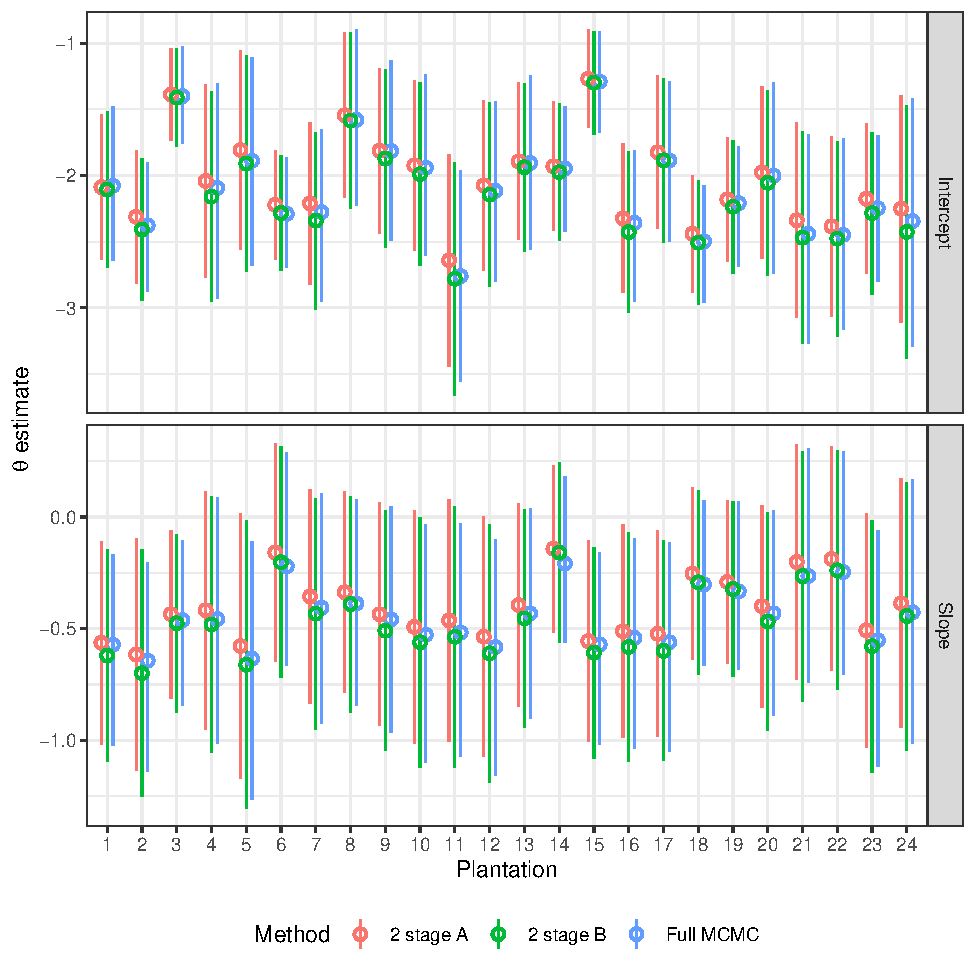
\includegraphics[width=6.5in]{plt_theta}
\caption{\label{fig:theta.re}Random effect inference for Example II using 2-stage and full MCMC methods. In the 2-stage analyses this was estimated using $\tilde{\bt}_i = \bX_i\tilde{\bb} + \tilde{u}_i$, where the tilde represents second stage estimates.}
\end{figure}

\clearpage

\begin{figure}
%\hspace*{-0.5in}
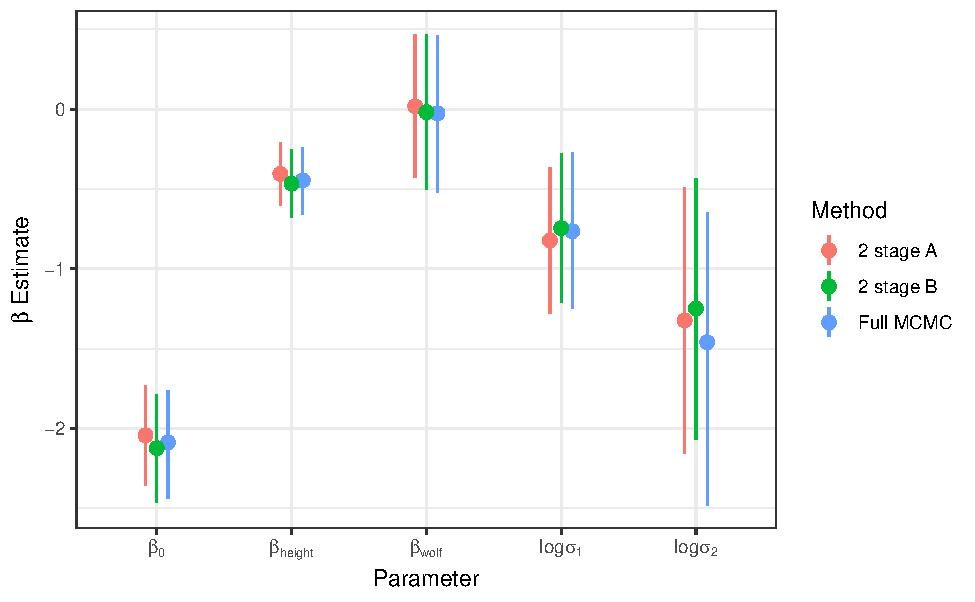
\includegraphics[width=6.5in]{fixpar}
\caption{\label{fig:fixed.re}Fixed effect and variance parameter inference for Example I using 2-stage and full MCMC methods.}
\end{figure}

\clearpage

\begin{figure}
%\hspace*{-0.5in}
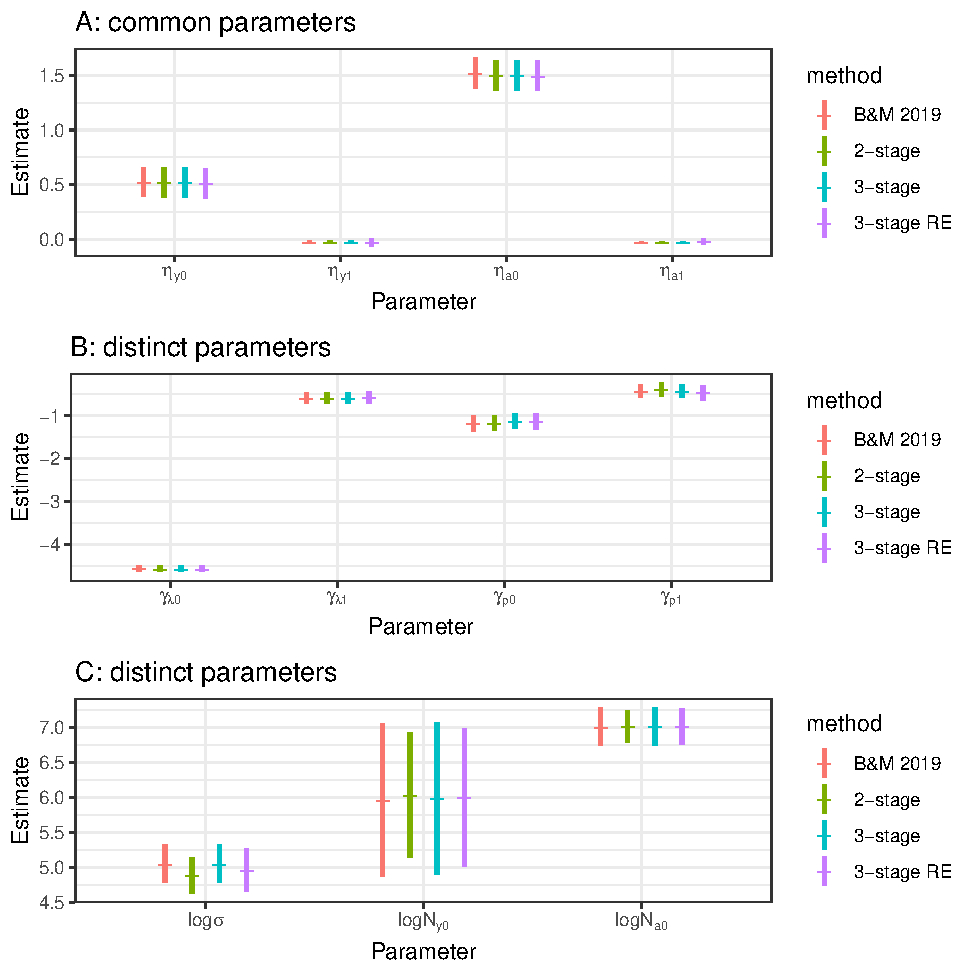
\includegraphics[width=6.5in]{effects_all} 
\caption{\label{fig:ipm} Parameter estimates for the lapwing IPM model. The B\&M 2019 results were taken from Table 2 of \citet{besbeas2019exact} and represent estimates from single stage estimation of the full model. In the 3-stage RE model, $\bn_i \sim N(\bn,\sigma_{\eta}\bI)$. Exact parameter estimates are provided in Appendix \ref{sec:ipm.results}}
\end{figure}


\clearpage

\begin{figure}
%\hspace*{-0.5in}
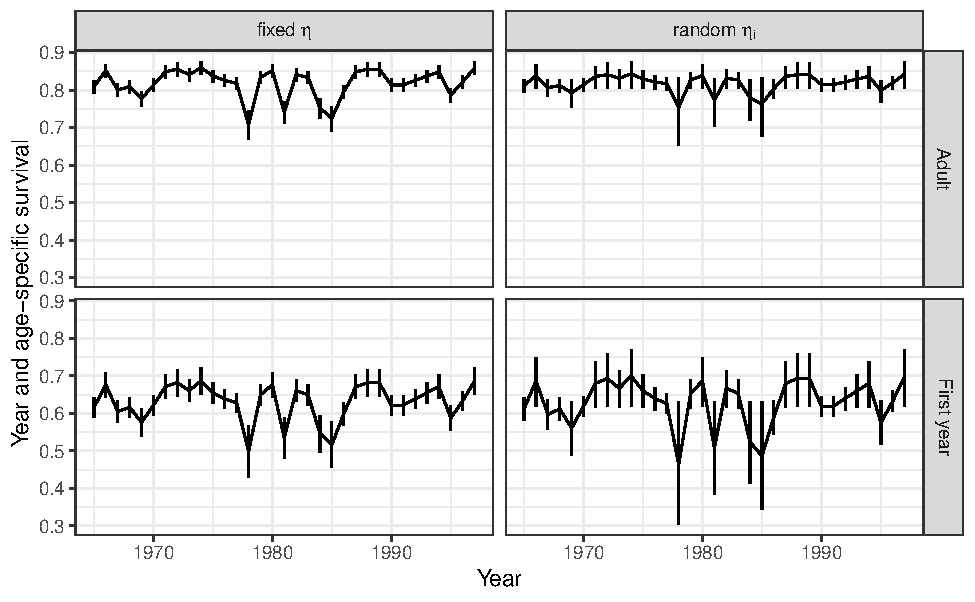
\includegraphics[width=6.5in]{survival} 
\caption{\label{fig:surv}Estimates of year and age-specific survival for lapwings. The different age classes are represented in the rows; adult and first year. The columns illustrate estimates from the two different models. The first column is the traditional IPM were the survival parameters are common between the data sets, i.e., $\bn$ is fixed. In the second column we modeled $\bn_i \sim N(\bn, \sigma_{\eta}^2\bI)$, where $\sigma_{\eta}$ is estimated in the second stage.}
\end{figure}

\clearpage

\appendix

\section{Deterministic Bayesian inference} 
\label{sec:methodii}

To this point we have only considered using the posterior mode and Hessian derived covariance matrix for the first stage normal approximation. For a large amount of data in the first stage, this might be just fine. But, we might consider using the posterior mean and variance of $\bt_i$ instead. If MCMC is used in the first stage, we can of course just calculate the sample mean and covariance matrix. If this is the case one might just as well use the two-stage MCMC procedures proposed and discussed by \cite{lunn2013fully}, \cite{hooten2018prior}, and \cite{goudie2019joining}. If the number of parameters is relatively small, say $\le 6$, we propose using a deterministic sampling procedure for approximating the posterior mean and variance (see \citealt{johnson2011bayesian}). 

The deterministic procedure proceeds as follows for each $i$,.
\begin{enumerate}
\item Maximize $[\bt|\by]$, to obtain the posterior mode, $\hat{\bt}$ and covariance matrix, $\hat{\bS}$
\item Form the Eigen decomposition of the covariance matrix $\hat{\bS} = \mathbf{V}\boldsymbol{\Lambda}\mathbf{V}'$
\item Explore the principle axes of $[\bt|\by]$ via the parameterization $\bt^{(j)} = \hat{\bt} + \mathbf{V}\boldsymbol{\Lambda}^{1/2}\mathbf{z}$, where $\mathbf{z}$ is successively incremented from $\mathbf{0}$ one entry at a time by step length, say $\delta_z$ until $\log[\hat{\bt}|\by]-\log[\bt^{(j)}|\by] > \delta_\pi$.
\item Repeat by successively incrementing each element of $\mathbf{z}$ by $-\delta_z$.
\item Finally, form a grid with every combination of the dimensionality $\bt^{(j)}$ entries saved in the previous two steps and retain with the same $\delta_\pi$ criterion.
\item Form weights $w_j \propto [\bt^{(j)}|\by]$
\end{enumerate}
The main benefit of the deterministic approach is that it avoids having to select a proposal distribution and assess chain convergence. The drawbacks of this approach, however, are the unknown number of likelihood evaluations and the potential coarseness in high density areas. As the number of parameters becomes large this method quickly succumbs to the curse of dimensionality.
\clearpage 

\section{Additional results for Example II: An integrated data model}
\label{sec:ipm.results}

\begin{table}[!h]
\caption{Full results for Example II: Integrated data modelThe B\&M 2019 results were taken from Table 2 of \citet{besbeas2019exact} and represent estimates from single stage estimation of the full model. In the 3-stage RE model, $\bn_i \sim N(\bn,\sigma_{\eta}\bI)$.} \medskip
\begin{tabular}{lllll}
\hline \hline
Parameter & B\&M 2019 & 2-stage & 3-stage & 3-stage RE\\
\hline
$\eta_{y0}$ & 0.523  ( 0.067 ) & 0.519  ( 0.068 ) & 0.519  ( 0.068 ) & 0.511  ( 0.070 )\\
$\eta_{y1}$ & -0.023  ( 0.007 ) & -0.024  ( 0.007 ) & -0.024  ( 0.007 ) & -0.03  ( 0.019 )\\
$\eta_{a0}$ & 1.521  ( 0.070 ) & 1.500  ( 0.068 ) & 1.500  ( 0.068 ) & 1.496  ( 0.070 )\\
$\eta_{a1}$ & -0.028  ( 0.005 ) & -0.028  ( 0.005 ) & -0.028  ( 0.005 ) & -0.017  ( 0.014 ) \bigskip\\
$\gamma_{\lambda 0}$ & -4.563  ( 0.035 ) & -4.566  ( 0.035 ) & -4.566  ( 0.035 ) & -4.568  ( 0.035 )\\
$\gamma_{\lambda 1}$ & -0.584  ( 0.064 ) & -0.582  ( 0.065 ) & -0.582  ( 0.065 ) & -0.573  ( 0.065 )\\
$\gamma_{\rho 0}$ & -1.178  ( 0.091 ) & -1.175  ( 0.087 ) & -1.115  ( 0.086 ) & -1.128  ( 0.091 )\\
$\gamma_{\rho 1}$ & -0.425  ( 0.076 ) & -0.388  ( 0.081 ) & -0.428  ( 0.077 ) & -0.456  ( 0.087 ) \bigskip \\
$\log \sigma$ & 5.049  ( 0.136 ) & 4.884  ( 0.127 ) & 5.052  ( 0.138 ) & 4.965  ( 0.152 )\\
$\log N_{y0}$ & 5.966  ( 0.546 ) & 6.039  ( 0.447 ) & 5.985  ( 0.547 ) & 6.001  ( 0.494 )\\
$\log N_{a0}$ & 7.015  ( 0.135 ) & 7.019  ( 0.114 ) & 7.016  ( 0.137 ) & 7.019  ( 0.126 )\\
$\log \sigma_\eta$&  & & & -4.062 (0.519)\\
\hline
\end{tabular}
\end{table}

\end{document}

